\documentclass[12pt, french]{article}

\usepackage{fancyhdr, fancybox, lastpage}
\usepackage[most]{tcolorbox}
\usepackage[a4paper, margin={0.3in, .75in}]{geometry}
\usepackage[siunitx, RPvoltages]{circuitikz}
\usepackage{wrapfig}
\pagestyle{fancy}
\renewcommand\headrulewidth{1pt}
\renewcommand\footrulewidth{1pt}
\fancyhf{}
\rhead{ \em{Zakaria Haouzan}}
\lhead[C]{\em{1ére année baccalauréat Sciences Mathématiques}}
\chead[C]{}
\rfoot[C]{}
\lfoot[R]{}
\cfoot[]{\em{Page \thepage / \pageref{LastPage}}}


\newtcolorbox{Box2}[2][]{
                lower separated=false,
                colback=white,
colframe=white!20!black,fonttitle=\bfseries,
colbacktitle=white!30!gray,
coltitle=black,
enhanced,
attach boxed title to top left={yshift=-0.1in,xshift=0.15in},
title=#2,#1}


\begin{document}
\begin{center}
   \shadowbox {\bf{Champ magnétique }}
\end{center}


%%_________________________Exercice ! :"_________________________Exercice
   \begin{Box2}{Exercice 1 :  les caractéristiques du champ magnétique  }
\begin{wrapfigure}{r}{0.3\textwidth}
  \begin{center}
     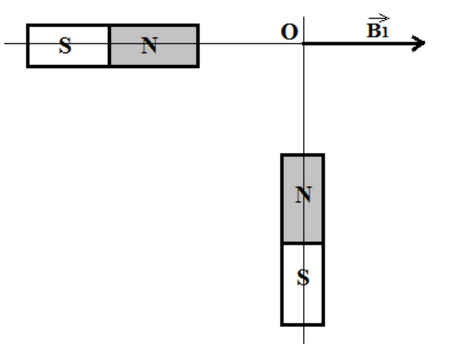
\includegraphics[width=0.2\textwidth]{./img/ex001.png}
  \end{center}
\end{wrapfigure}
      Une aiguille dont le centre O est placé sur l’axe de l’aimant 1 s’aligne sur cet axe suivant le vecteur $\vec{B_1}$de valeur $5,0 mT$. 

      On place l’aimant 2 comme c’est montrer sur la figure : l’aiguille tourne dans le sens
contraire des aiguilles d’une montre d’un angle $\alpha = 24$°.

Déterminer les caractéristiques du champ magnétique $\vec{B_2}$ créé en O par l’aimant 2 ainsi que les caractéristiques du champ magnétique résultant $\vec{B_T}$.

   \end{Box2}


%%_________________________Exercice !2 :"_________________________Exercice
\begin{Box2}{Exercice 2 :les caractéristiques du champ magnétique en un point  }
\begin{wrapfigure}{r}{0.5\textwidth}
  \begin{center}
     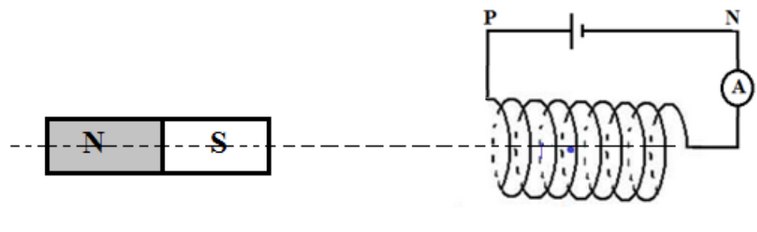
\includegraphics[width=0.48\textwidth]{./img/ex02.png}
  \end{center}
\end{wrapfigure}

Un aimant droit crée en un point P à l’intérieur d’un solénoïde de 140 spires et de longueur $16 cm$ un

   champ magnétique de valeur $2,5 mT$. 

   Déterminer le sens et l’intensité du courant électrique qui va annuler
le champ magnétique en P.
\end{Box2}

%%_________________________Exercice ! 3:"_________________________Exercice
\begin{Box2}{Exercice 3 :  bobine parcourue par un courant I}


   Une bobine parcourue par un courant d’intensité I, crée en M un champ magnétique de norme $B_1$=$2mT$.
Un aimant A crée au même point un champ magnétique de norme $B_2=4mT$.

1. Représenter les vecteurs champ magnétique créés en M par chacune des deux sources.

2. Représenter le vecteur champ magnétique résultant.

3. Déterminer sa norme
  \begin{center}
     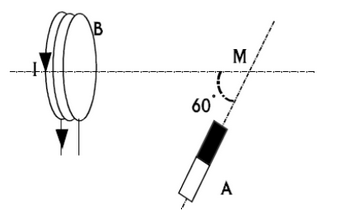
\includegraphics[width=0.48\textwidth]{./img/exo03.png}
  \end{center}

\end{Box2}
\begin{center}

   \vspace{4cm}
   \Large{ \em{Exercices Supplémentaires}}
\end{center}


\begin{Box2}{Exercice 4 :Champ magnétique créé par un courant électrique  }
1.On considère deux barreaux aimantés $A_1$ et $A_2$ posés sur le même alignement avec un point M comme l'indique la
figure (1).

Sachant que les intensités des champs magnétiques créés par A1 et A2 au point M sont : $B_1=20mT$ et $B_2=30mT$.

2.Représenter les vecteurs champ magnétique en utilisant l'échelle suivante $1cm ->10mT$.Puis représenter le vecteur champ magnétique globale au point M.

3.Déterminer graphiquement puis par calcul l'intensité du champ magnétique 
   global au point M, puis déterminer l'angle que forme $\vec{B}$ avec le plan horizontal.(On néglige le champ magnétique terrestre.)
  \begin{center}
     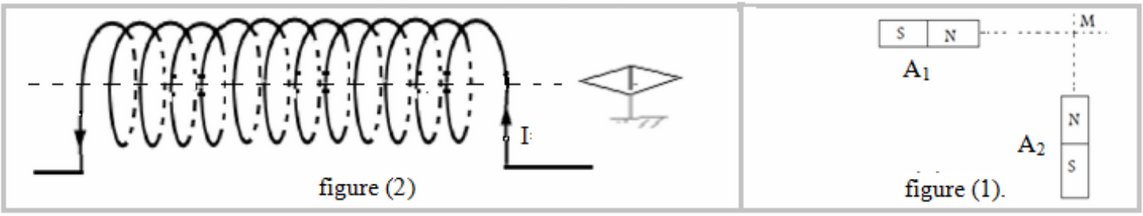
\includegraphics[width=0.85\textwidth]{./img/Exo__sol.png}
  \end{center}
4.On considère une bobine de rayon $R=2,5cm$ et de longueur $L=60cm$ composée de $N=600$ spires et parcourue par un courant électrique d'intensité $I=239mA$ comme l'indique la figure (2).

4.1 Donner la définition d'un solénoïde.

   4.2 Montrer la bobine précédente peut être considérée comme un solénoïde.

   4.3 Déterminer l'intensité du champ magnétique crée par ce solénoïde.

   4.4 Préciser la nature de chacune des faces du solénoïde.

   4.5 Préciser les pôles de l'aiguille aimantée.

   4.6  Déterminer le sens et la direction du champ magnétique $\vec{B}$ créé par le solénoïde à l'intérieur.

   4.7 Représenter le spectre du champ magnétique créé par le solénoïde.(0,5pt)

   4.8 Sachant que le diamètre du fil enroulé d=2mm, quelle est le nombre de couches enroulées sur le cylindre formant le solénoïde

   \begin{wrapfigure}{r}{0.2\textwidth}
  \begin{center}
     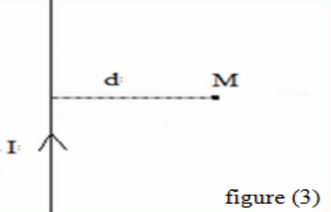
\includegraphics[width=0.2\textwidth]{./img/Exo_fil.png}
  \end{center}
\end{wrapfigure}


   5. On considère un long conducteur rectiligne parcouru par un courant électrique d'intensité I=12A comme l'indique la
figure (3) :

5.1. Donner l'expression du champ magnétique créé par le conducteur au point M

5.2. Représenter Le vecteur champ magnétique créé par le conducteur au point M.

5.3. Calculer l'intensité du champ magnétique créé par le conducteur au point M on donne d=2mm.

\end{Box2}

%%%_________________________Exercice 4 : _________________________Exercice
%\begin{Box2}{Exercice 5 : les paramètres d’une pile }
%\begin{wrapfigure}{r}{0.3\textwidth}
  %\begin{center}
     %\vspace{-0.5cm}
    %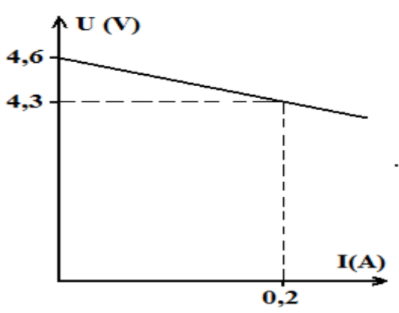
\includegraphics[width=0.3\textwidth]{./img/carcateristique_generateur.png}
  %\end{center}
%\end{wrapfigure}
  
   %Au cours d’une séance de travaux pratiques, on détermine les paramètres (E, r) d’une pile de 4,5V en traçant sa
%caractéristique intensité - tension.

%1. Proposer un montage électrique pour tracer cette caractéristique. On dispose de la pile, d’une résistance variable (0-100$\Omega$ ; 0-2 A), de deux multimètres et d’un interrupteur.
%Faites apparaître sur ce circuit les deux bornes de chaque multimètre, la flèche de la tension mesurée ainsi que
%l’intensité du courant.

   %On a la courbe suivantes.En déduire la force électromotrice E et la résistance interne r de cette pile. Justifier.

   %2. Pour une tension U = 4,21 V, déterminer :
%\\a. La puissance électrique fournit au circuit extérieur.
%\\b. La puissance chimique transformée en puissance électrique.
%\\c. La puissance dissipée sous forme d’effet Joule dans la pile.
%3) Faire un schéma énergétique montrant les transferts d’énergie s’effectuant au niveau de la pile.
%\end{Box2}
%%\vspace{2cm}
%%%_________________________Exercice 5 : _________________________Exercice
%\begin{Box2}{Exercice 6 : bilan énergétique}
%\begin{wrapfigure}{r}{0.4\textwidth}
  %\begin{center}
     %\vspace{-0.5cm}
    %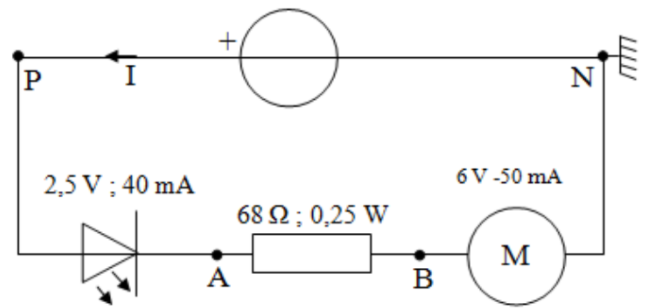
\includegraphics[width=0.4\textwidth]{./img/diode_circuit.png}
  %\end{center}
%\end{wrapfigure}
%On réalise le circuit suivant :
   %\\- $U_{PN}=12,16 V$
%\\- $I=48 mA$
   %\\- $U_{PA}=2,62 V$
   %\\- $U_{AB}=3,28 V$
   %\\- $U_{BN}=6,28 V$

   %On règle le générateur sur 12 V continue

   %1. Que signifient les valeurs indiquées au-dessus de chaque récepteur ?

   %2. Flécher sur le schéma les tensions UPN, UPA, UAB et UBN. Mesurer chacune d’entre elle.

   %3. Mesurer l’intensité du courant qui est débitée par le générateur.

   %4. Que dire du courant qui circule dans les récepteurs ? Le vérifier par une mesure pour le moteur

   %5. Exprimez puis calculer l’énergie électrique E (en J) fournie au circuit par le générateur pendant
%1minute.

   %6. Exprimez puis calculer les énergies électriques E1, E2, E3 reçues respectivement par la DEL, la
%résistance et le moteur pendant cette même durée.

   %7. Quelle est la relation littérale qui lie E, E1, E2, E3 ? La vérifier numériquement.

   %8. En déduire, à partir de ce bilan énergétique, la relation entre UPN, UPA, UAB et UBN. Vérifier la relation numériquement.
%\end{Box2}
%%%_________________________Exercice 6 : _________________________Exercice
\end{document}
